%\documentclass{clases}
\documentclass[a4paper,12pt, oneside]{book}
\usepackage[skins,minted]{tcolorbox}
\usepackage[utf8]{inputenc}
\usepackage[T1]{fontenc}
\usepackage[spanish, es-tabla]{babel}
\languageshorthands{spanish}
%\usepackage{lmodern} % Usa las fuentes modernas de LaTeX
\usepackage[numbers]{natbib}
%\usepackage{morewrites}
\usepackage{inconsolata}
\usepackage{mdframed}
\usepackage{minted}
\usepackage{bm}
\usepackage{listingsutf8}
\usepackage{subcaption}
\usepackage{amsmath}
\usepackage{amssymb}
\usepackage{graphicx}
\usepackage{hyperref}
\usepackage{longtable}
\usepackage{tabularx}
\usepackage{threeparttable}
\usepackage{array}    % Necesario para centrar horizontal y verticalmente
\usepackage{xcolor}
\usepackage{pdfpages}
%\usepackage{color}
\usepackage{fancyhdr}
\usepackage{menukeys}
\usepackage{appendix}
\usepackage{fontawesome}
\usepackage{comment}
\usepackage{caption}
\usepackage{setspace}
\usepackage[explicit]{titlesec}
\usepackage[a4paper,margin=2cm]{geometry}

%\geometry{top=3cm, bottom=3cm, left=4cm, right=2cm} % Si lo quieres imprimir

\definecolor{green1}{HTML}{1dae28}
\definecolor{green2}{HTML}{afd095}
\definecolor{lightgray}{gray}{0.9}
\definecolor{orange}{RGB}{18,84,183}
\definecolor{titulo}{gray}{0.75}
\definecolor{gray97}{gray}{.97}
\definecolor{gray75}{gray}{.75}
\definecolor{gray45}{gray}{.45}
\definecolor{advertencia}{RGB}{255,178,102}
\definecolor{colorturqueza}{RGB}{178,223,238}
\definecolor{mintedbackground}{rgb}{0.95,0.95,0.95}
\definecolor{lbcolor}{rgb}{0.95,0.95,0.95}
\definecolor{mintedframe}{rgb}{0.0,0.0,0.0}
\definecolor{codebg}{rgb}{0.96,0.96,0.96}
\definecolor{colorurls}{RGB}{107,17,17}
\definecolor{colorsql}{RGB}{255,245,245}
\definecolor{colorreferences}{RGB}{48,134,3}
\definecolor{titulo}{gray}{0.65}			%------ color para fondo del titulo de tablas.

\hypersetup{
	%bookmarks=true,         % show bookmarks bar?
	unicode=true,          % non-Latin characters in Acrobat’s bookmarks
	pdftoolbar=true,        % show Acrobat’s toolbar?
	pdfmenubar=true,        % show Acrobat’s menu?
	pdffitwindow=false,     % window fit to page when opened
	pdfstartview={FitH},    % fits the width of the page to the window
	pdftitle={Reporte final de Robótica},    % title
	%	pdfauthor={},     % author
	pdfsubject={Reporte final de Robótica},   % subject of the document
	%pdfcreator={pdfTeX 3.14159265-2.6-1.40.16 (TeX Live 2016/dev)},   % creator of the document
	%pdfproducer={Panel HJ 2017}, % producer of the document
	pdfkeywords={Manipulador industrial} {Robotica} {ros} {gazebo}, % list of keywords
	%pdfnewwindow=true,      % links in new PDF window
	colorlinks=true,       % false: boxed links; true: colored links
	linkcolor=black,          % color of internal links (change box color with linkbordercolor)
	citecolor=colorreferences,        % color of links to bibliography
	filecolor=magenta,      % color of file links
	urlcolor=blue,           % color of external links
	linkbordercolor={0 0 0}
}

\lstset{
	inputencoding=utf8,
	language=Python,
	frame=Ltb,
	tabsize=2,
	framerule=0pt,
	aboveskip=0.5cm,
	framextopmargin=0pt,
	framexbottommargin=0pt,
	framexleftmargin=0.4cm,
	framesep=0pt,
	rulesep=.0pt,
	backgroundcolor=\color{gray97},
	rulesepcolor=\color{blue},
	%
	stringstyle=\ttfamily,
	showstringspaces = false,
	basicstyle=\small\ttfamily,
	commentstyle=\color{gray45},
	keywordstyle=\bfseries,
	%
	numbers=none,
	numbersep=15pt,
	numberstyle=\tiny,
	numberfirstline = false,
	breaklines=true
}

\setminted[bash]{
	bgcolor=mintedbackground,
	fontfamily=tt,
	linenos=true,
	numberblanklines=true,
	numbersep=11pt,
	numbersep=2pt,
	gobble=0,
	frame=leftline,
	framesep=2mm,
	funcnamehighlighting=false,
	tabsize=4,
	obeytabs=false,
	samepage=false,
	showspaces=false,
	showtabs =false,
	texcl=false,
	baselinestretch=1.2,
	fontsize=\footnotesize,
	breaklines=true,
	breaksymbolleft=\ 
}
%\setminted{%
%	breaklines,
%	breaksymbolleft=,      % vacía la marca de continuación
%	breaksymbolright=      % también limpia el símbolo a la derecha
%}


\lstdefinestyle{consola}{
	basicstyle=\footnotesize\bf\ttfamily,
	backgroundcolor=\color{gray75},
}	
\definecolor{gray}{rgb}{0.4,0.4,0.4}
\definecolor{darkblue}{rgb}{0.0,0.0,0.6}
\definecolor{cyan}{rgb}{0.0,0.6,0.6}
\lstset{language=XML}

\lstdefinelanguage{XML}{
	morestring=[b]",
	tabsize=2,
	breaklines=true,
	morestring=[s]{>}{<},
	morecomment=[s]{<?}{?>},
	stringstyle=\color{black},
	identifierstyle=\color{darkblue},
	keywordstyle=\color{cyan},
	numbers=left,
	morekeywords={xmlns,version,type}% list your attributes here
}

\lstdefinestyle{C}{language=C}
\lstdefinestyle{XML}{language=XML}

\DeclareMathOperator{\diag}{diag}

\newtcblisting{terminal}[2][]{
	listing engine=minted,
	listing only,
	#1,
	title=#2,
	minted language=bash,
	colback=mintedbackground,
	top=0mm,
	bottom=0mm
}

\newtcblisting{consolestyle}[2][]{enhanced, listing engine=minted, 
	listing only,#1, title=#2, minted language=bash, 
	coltitle=mintedbackground!35!black, 
	fonttitle=\ttfamily\footnotesize,
	sharp corners, top=0mm, bottom=0mm,
	title code={\path[draw=mintedframe, dashed, fill=mintedbackground](title.south west)--(title.south east);},
	frame code={\path[draw=mintedframe, fill=mintedbackground](frame.south west) rectangle (frame.north east);}
}

\newenvironment{doble}
{\doublespacing
}

%\newcounter{comando}[section]
%\newenvironment{comando}[1][]{\refstepcounter{comando}\par\medskip
	%	\noindent \textbf{Comando~\thecomando. #1} \rmfamily}{\medskip}
%\begin{terminal}{#1}

%\end{terminal}
%}{\medskip}

\graphicspath{{img/}{tablas/}{portada/}}  % Las imágenes se buscarán en la carpeta "img"

\addto\captionsspanish{\renewcommand{\contentsname}{Índice}}

\def\CC{{C\nolinebreak[4]\hspace{-.05em}\raisebox{.4ex}{\tiny\bf ++ \space}}}
\def\Cc{{C\nolinebreak[4]\hspace{-.05em}\raisebox{.4ex}{\tiny\bf ++}}}
\newcommand{\ffolder}[1]{\menu{\faFolderO \space #1}}
\newcommand{\ffile}[1]{\menu{\faFileO \space #1}}
\newcommand{\folder}{\faFolderO \space}
\newcommand{\file}{\faFileO \space}
\newcommand{\world}{\faGlobe \space}
\newcommand{\wworld}[1]{\menu{\faGlobe \space #1}}
\newcommand{\SB}{\{B\}} % Define el sistema del cuerpo
\newcommand{\SI}{\{I\}} % Define el sistema inercial

\newcounter{actividad} % Define un contador llamado "actividad"

\newfloat{Comando}{h}{lot}[chapter]

\renewcommand{\tablename}{Tabla}
\renewcommand{\listtablename}{Índice de tablas}
\renewcommand\listingscaption{Código}
\newcommand{\code}[1]{\colorbox{lightgray}{\texttt{#1}}}

\renewcommand\lstlistingname{Código}
\renewcommand{\appendixname}{Anexo}
\renewcommand{\appendixtocname}{Anexos}
%\renewcommand{\appendixpagename}{Anexo}
\renewcommand\labelitemi{$\bullet$}

\begin{document}
	% Aquí se encuentra el archivo con la portada
	\begin{titlepage}
	\centering
	%-------------------------------------------
	% Logos en una tabla: izquierda, centro y derecha
	\begin{tabular}{@{}p{0.3\textwidth} p{0.3\textwidth} p{0.3\textwidth}@{}}
		
\includegraphics[height=2cm]{tecnm} & 
		\centering 
\includegraphics[height=1.5cm]{SEP} & 
		\raggedleft 
\includegraphics[height=2cm]{ith.jpg} \\
	\end{tabular}
	
	\vspace{2em}
	
	\noindent
	%-------------------------------------------
	%	Información institucional y académica (esquina superior izquierda)
	\begin{minipage}[t]{0.48\textwidth}
		\raggedright
		\small \textbf{%
			Instituto Tecnológico de Hermosillo\\
			Materia: Robótica\\
			Profesor: Medina Gil Lamadrid, Jesús Iván%
		}
	\end{minipage}%
	\hfill
	%	fecha actual (esquina superior derecha), en letras pequeñas y en negrita.
	\begin{minipage}[t]{0.48\textwidth}
		\raggedleft
		\small \textbf{\today}
	\end{minipage}
	
	\vspace{2em}
	
	%-----------------------------------------
	% Unidad y Título de la tarea en letras grandes y en negrita
	{\large \textbf{Unidad 1: Morfología del robot}}\\
	{\Huge \textbf{Investigar sobre diferentes tipos de sensores}}
		
	\vspace{1em}
	
	%---------------------------------------
	% Tabla con la información del equipo
	%---------------------------------------
	% Encabezado del equipo
	\begin{center}
		{\Large \textbf{Equipo 4}}
	\end{center}
	
	\vspace{1em}
	
	% Tabla de integrantes:
	% Cada fila contiene: foto (columna izquierda) y datos del integrante (columna derecha)
	\begin{center}
		\begin{tabular}{c c}
			\begin{tabular}{c}
				
\includegraphics[height=3cm]{perfil1.jpg} \\
				\textbf{Fuentes Ochoa},\\ Aislinn Alicia \\ \texttt{l21330583@hermosillo.tecnm.mx} \\ Teléfono: 6371147080
			\end{tabular} &
			\begin{tabular}{c}
				
\includegraphics[height=3cm]{perfil2.jpg} \\
				\textbf{Gonzalez Cueto,}\\ Alejandra Abigail \\ \texttt{l21330591@hermosillo.tecnm.mx} \\ Teléfono: 6221223887
			\end{tabular} \\ \vspace{2em}
			\begin{tabular}{c}
				
\includegraphics[height=3cm]{perfil3.jpg} \\
				\textbf{Ceballos Portillo,}\\ Patsy \\ \texttt{l21330551@hermosillo.tecnm-mx} \\ Teléfono: 6622968916
			\end{tabular} &
			\begin{tabular}{c}
				
\includegraphics[height=3cm]{perfil4.jpg} \\
				\textbf{Peña Encinas}\\ Ana Lourdes \\ \texttt{l21331075@hermosillo.tecnm.mx} \\ Teléfono: (6621281812)
			\end{tabular}
		\end{tabular}
	\end{center}

\end{titlepage}

	\onehalfspacing
	\frontmatter
	\pagestyle{plain}  % numeración en páginas preliminares
	\titleformat{\chapter}
	{\bfseries\huge}
	{}
	{0pt}
	{~\raisebox{-1.5pt}{}
	\\\filleft #1 \\\vspace{.25cm}\titlerule[1.5pt]}
	
	% ---------------------------------------
	% índices
%	\clearpage   % o \cleardoublepage, según prefieras
	\newpage
	\phantomsection    % crea un nuevo destino para hyperref
	\addcontentsline{toc}{chapter}{Índice general}
	\tableofcontents
	
%	\clearpage
	\newpage
	\phantomsection
	\addcontentsline{toc}{chapter}{Índice de figuras}
	\listoffigures
	
	\hypersetup{
		linkcolor=red
	}
	
	% ---------------------------------------
	% Estilo de encabezado y pie de página
	\mainmatter
	\pagestyle{fancy}
	\fancyhead{}
	\fancyhead[L]{\leftmark}
	\fancyhead[R]{}
	\fancyfoot[L]{\parbox[l]{\textwidth-1cm}{\rightmark}}
	\fancyfoot[C]{}
	\fancyfoot[R]{\thepage}
	\renewcommand{\footrulewidth}{0.5pt}
	%\fancyfoot[RO,LE]{Diseño de modelo para simulación 3D de VANT tipo cuadricóptero}
	
	\titleformat{\chapter}
	{\bfseries\huge}
	{}
	{0pt}
	{\titlerule[3pt]~\raisebox{-1.5pt}{\sc{\chaptername}~\thechapter}~\titlerule[3pt]%
		\\\vspace{.05cm}\titlerule\\\filcenter #1 \\\vspace{.25cm}\titlerule}
	
	% Capítulo 1: Introducción
	\chapter{Marco Teórico} 
\label{chap:marco_teorico}

La robótica es una rama de la ingeniería que estudia el diseño, construcción, operación y aplicación de robots, así como los sistemas computacionales que los controlan. Un robot es una máquina reprogramable capaz de realizar una serie de acciones automáticamente o por control externo, con cierto grado de autonomía. El estudio de los robots implica diversas áreas del conocimiento, entre ellas la mecánica, la electrónica, la programación y la teoría del control.

La cinemática se encarga del estudio del movimiento de los cuerpos sin considerar las fuerzas que los causan. En robótica, se distingue entre:

\textbf{Cinemática directa:} determina la posición y orientación del efector final en función de los valores articulares.

\textbf{Cinemática inversa:} calcula los valores articulares necesarios para alcanzar una posición deseada del efector.


El análisis cinemático es esencial para programar tareas de posicionamiento precisas en robots manipuladores.

La dinámica estudia el comportamiento del robot considerando las fuerzas involucradas en su movimiento. Permite calcular los torques o fuerzas necesarias para lograr un cierto movimiento bajo condiciones dinámicas. Este análisis es fundamental para el diseño del sistema de control y para garantizar que el robot pueda ejecutar tareas de manera estable y segura.
Las propiedades dinámicas de un robot incluyen:

\textbf{Inercia:} resistencia de las masas del robot al cambio de movimiento.

\textbf{Centrífugas y coriolis:} fuerzas que aparecen en sistemas en movimiento.

\textbf{Par gravitacional:} el efecto del peso del robot sobre sus articulaciones.

\cite{fundamentosRobotica}
\cite{introduccionRobotica}





	
	% Capítulo 2: Marco Teórico
	\chapter{Marco Teórico} 
\label{chap:marco_teorico}

La robótica es una rama de la ingeniería que estudia el diseño, construcción, operación y aplicación de robots, así como los sistemas computacionales que los controlan. Un robot es una máquina reprogramable capaz de realizar una serie de acciones automáticamente o por control externo, con cierto grado de autonomía. El estudio de los robots implica diversas áreas del conocimiento, entre ellas la mecánica, la electrónica, la programación y la teoría del control.

La cinemática se encarga del estudio del movimiento de los cuerpos sin considerar las fuerzas que los causan. En robótica, se distingue entre:

\textbf{Cinemática directa:} determina la posición y orientación del efector final en función de los valores articulares.

\textbf{Cinemática inversa:} calcula los valores articulares necesarios para alcanzar una posición deseada del efector.


El análisis cinemático es esencial para programar tareas de posicionamiento precisas en robots manipuladores.

La dinámica estudia el comportamiento del robot considerando las fuerzas involucradas en su movimiento. Permite calcular los torques o fuerzas necesarias para lograr un cierto movimiento bajo condiciones dinámicas. Este análisis es fundamental para el diseño del sistema de control y para garantizar que el robot pueda ejecutar tareas de manera estable y segura.
Las propiedades dinámicas de un robot incluyen:

\textbf{Inercia:} resistencia de las masas del robot al cambio de movimiento.

\textbf{Centrífugas y coriolis:} fuerzas que aparecen en sistemas en movimiento.

\textbf{Par gravitacional:} el efecto del peso del robot sobre sus articulaciones.

\cite{fundamentosRobotica}
\cite{introduccionRobotica}





	
		\section{Cinemática} \label{sec:cinematica}

Explicar su definición en base a lo que viene en libros o de los archivos de Matlab. Diferenciar entre \textbf{Cinemática directa} y \textbf{Cinemática inversa}.
Para el proceso sobre cómo se llevó a cabo el algoritmo en Matlab, ir a la  \hyperref[sec:proceso_cinematica]{sección del proceso de Cinemática}.

\subsection{Cinemática Directa}
Explicar sobre la definición geométrica usando Denavit Hartenberg con el algoritmo y las matemáticas.

\subsection{Cinemática Diferencial}
Aquí explicarán sobre el jacobiano para la cinemática diferencial.

\subsection{Cinemática Inversa}
Explicar su definición y cómo se relaciona el gradiente con el jacobiano. Cabe destacar que existen multitud de métodos y en mi clase solo usaron un método, pero aquí pueden explicar las imágenes que vienen en Matlab.


		
		\section{ROS} \label{sec:ros}
ROS, cuyas siglas significan Robot Operating System, es un framework de software ampliamente utilizado en el desarrollo de aplicaciones robóticas. Aunque se le llama “sistema operativo”, ROS en realidad no es un sistema operativo completo como Windows o Linux, sino un conjunto de bibliotecas, herramientas y convenciones diseñadas para facilitar la creación de software para robots.


ROS proporciona una infraestructura flexible que permite a los desarrolladores crear sistemas robóticos complejos de forma modular, escalable y colaborativa. Esto se logra mediante la creación de nodos independientes que se comunican entre sí a través de un sistema de mensajes. Cada nodo puede encargarse de tareas específicas, como leer sensores, controlar motores, planear trayectorias o tomar decisiones, y todos estos módulos pueden intercambiar información de forma sincronizada en tiempo real. 
\cite{lovtechnology2024}


\begin{figure}[h]
	\centering
	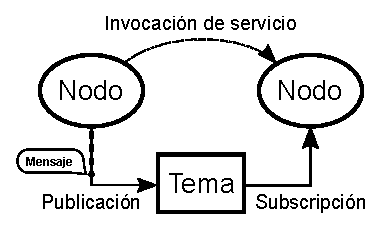
\includegraphics[width=0.5\linewidth]{img/ROS_concepts}
	\caption{Diagrama de comunicación de ROS}
	\label{fig:rosconcepts}
\end{figure}

Uno de los aspectos más importantes de ROS es su capacidad para abstraer la complejidad del hardware, lo que significa que los programadores pueden centrarse en la lógica y el comportamiento del robot sin preocuparse directamente por los detalles técnicos de cada componente físico. Gracias a esto, ROS ha sido adoptado en todo el mundo tanto en entornos académicos como industriales, y ha impulsado el desarrollo de robots móviles, brazos manipuladores, drones, vehículos autónomos, entre muchos otros.


\subsection{Nodo (Node)}

En el contexto de ROS (Robot Operating System), un nodo representa una unidad ejecutable que realiza una tarea específica dentro del sistema robótico. ROS está diseñado como un sistema distribuido, lo que significa que las tareas no se ejecutan en un único programa grande, sino que se dividen en varios nodos que pueden operar de forma independiente pero cooperativa. Por ejemplo, un nodo puede encargarse de leer datos de un sensor, otro puede controlar un motor, y un tercero puede realizar cálculos para la planificación de trayectorias. Esta arquitectura modular permite el desarrollo más organizado, reutilizable y escalable. Además, los nodos pueden ejecutarse en diferentes dispositivos conectados en red, lo que hace posible distribuir el procesamiento entre varios sistemas físicos.

\subsection{Tema (Topic)}
En ROS (Robot Operating System), un tópico es un canal de comunicación utilizado para el intercambio de mensajes entre nodos de forma asíncrona. A través de este mecanismo, un nodo puede publicar datos que otros nodos pueden recibir si están suscritos al mismo canal, sin necesidad de que haya una conexión directa entre ellos. Esto permite una arquitectura flexible y modular en la que distintos componentes del sistema pueden operar de manera independiente, facilitando el desarrollo y la escalabilidad de los proyectos. 

Por ejemplo, un nodo que lee datos de un sensor LiDAR puede publicar esa información constantemente en un tópico llamado "scan", mientras otros nodos, como los encargados del mapeo o de la detección de obstáculos, se suscriben a ese mismo tópico para procesar los datos en tiempo real. Esta comunicación basada en tópicos favorece la separación de responsabilidades entre nodos y permite que distintas partes del sistema se desarrollen, prueben o actualicen sin afectar a las demás, siempre y cuando se mantenga la estructura del mensaje. Además, ROS permite monitorear los tópicos en uso, visualizar qué nodos están publicando o suscribiéndose, y verificar que la información fluya correctamente dentro del sistema.
\subsection{Mensaje (Message)}
Los mensajes en ROS son las estructuras de datos que se intercambian entre nodos mediante tópicos o servicios. Cada mensaje tiene un tipo específico que define su estructura interna, como enteros, números decimales, cadenas de texto, o datos más complejos como vectores de posición y orientación. Por ejemplo, el mensaje "geometry msgs Twist" se usa para representar velocidades lineales y angulares, comúnmente utilizadas para controlar robots móviles. ROS proporciona una amplia variedad de tipos de mensajes predefinidos, pero también permite crear mensajes personalizados según las necesidades del proyecto. La estandarización de los mensajes es clave para que los nodos puedan interpretar correctamente los datos que reciben, facilitando la interoperabilidad entre módulos de distintos desarrolladores o bibliotecas.

\subsection{Servicio (Service)}
Un servicio en ROS representa una forma de comunicación sincrónica entre nodos, que sigue el esquema de solicitud-respuesta. A diferencia de los tópicos, que transmiten datos de forma continua, los servicios son adecuados para tareas que deben realizarse de forma puntual y donde se espera una respuesta inmediata. Por ejemplo, un nodo podría pedirle a otro que encienda un actuador, que cambie de modo de operación o que le proporcione la configuración de un sensor. Cada servicio tiene asociado un tipo de mensaje de solicitud y otro de respuesta, lo cual permite definir estructuras de datos precisas para cada operación. El uso de servicios es ideal cuando se necesita una interacción directa y controlada entre procesos dentro del sistema robótico.


\subsection{Gazebo}
Gazebo es un entorno de simulación tridimensional que se utiliza en conjunto con ROS para probar robots en escenarios virtuales antes de implementarlos en el mundo real. Este simulador proporciona una representación física realista que incluye elementos como gravedad, colisiones, fricción, inercia, y respuesta a fuerzas, lo cual permite una evaluación precisa del comportamiento de un robot bajo condiciones específicas. Gazebo es ampliamente utilizado en investigación, desarrollo y educación, ya que permite experimentar sin dañar hardware costoso. Además, permite simular una gran variedad de sensores como cámaras, LiDAR, GPS, IMUs, entre otros. La integración con ROS facilita que los nodos que se usan para controlar un robot real también puedan usarse sin modificaciones para controlar un robot virtual dentro de Gazebo, promoviendo así el desarrollo paralelo de software y hardware.

\subsection{RViz}
RViz (abreviación de "ROS Visualization") es una herramienta gráfica que permite visualizar información del sistema robótico en tiempo real. A través de RViz, los desarrolladores pueden ver modelos tridimensionales del robot, datos de sensores como cámaras o escáneres láser, trayectorias de movimiento, fuerzas, marcos de referencia (frames), mapas generados, y mucho más. Esta herramienta es extremadamente útil para depurar errores en el sistema, ya que permite comprobar si los datos están siendo generados correctamente y cómo se están interpretando dentro del entorno ROS. RViz se convierte en una interfaz visual intuitiva que ayuda a interpretar el estado interno del robot, facilitando la validación de algoritmos y el análisis del comportamiento general del sistema.

		
		\section{Dinámica} \label{sec:dinamica}

La verdad, no les expliqué mucho sobre esta unidad, pero pueden hablar sobre las ecuaciones que vienen en el powerpoint (el cual subí tarde porque se me corrompió)

Hablen sobre el modelo dinámico estandar de un robot, la matriz de masa o inercia, la matriz de coriolis y el vector de gravedad. 

\subsection{Matriz de masa o inercia}
Expliquen cómo el vector de masa o inercia define la aceleración máxima.

\subsection{Matriz de coriolis}

\subsection{Vector de gravedad}

Expliquen por qué el vector de gravedad en su valor máximo (cuando el robot está extendido horizontalmente) debe ser contrarrestado con la fuerza de cada motor

\subsection{Fricción}
Expliquen qué es la fricción en general.

\subsubsection{Fricción estática o seca}

\subsubsection{Fricción dinámica o viscosa}

\subsection{Perturbaciones}
Aquí expliquen qué es una perturbación en general sin profundizar mucho.
		
		\section{Control}
El diagrama de control de un robot industrial representa cómo se procesa la información desde que el usuario define lo que quiere que haga el robot, hasta que este ejecuta el movimiento real. Se puede dividir en tres bloques principales: la planificación de trayectoria, la cinemática inversa y la dinámica del robot.

Primero, el usuario define los valores que quiere que alcance el efector final del robot. Estos valores pueden ser las coordenadas de los puntos que debe seguir, la velocidad máxima, la aceleración máxima y el tipo de trayectoria. Esta información entra al bloque de planificación de trayectoria, donde se generan los valores que describen cómo debe moverse el efector final, como su posición, velocidad y aceleración, tanto lineal como angular.

Luego, esta información pasa a la parte de la cinemática inversa. Ahí se transforma en variables articulares, es decir, se calculan las posiciones, velocidades y aceleraciones que deben tener las articulaciones del robot para que el efector final logre seguir correctamente la trayectoria deseada.



\begin{figure}[h]
	\centering
	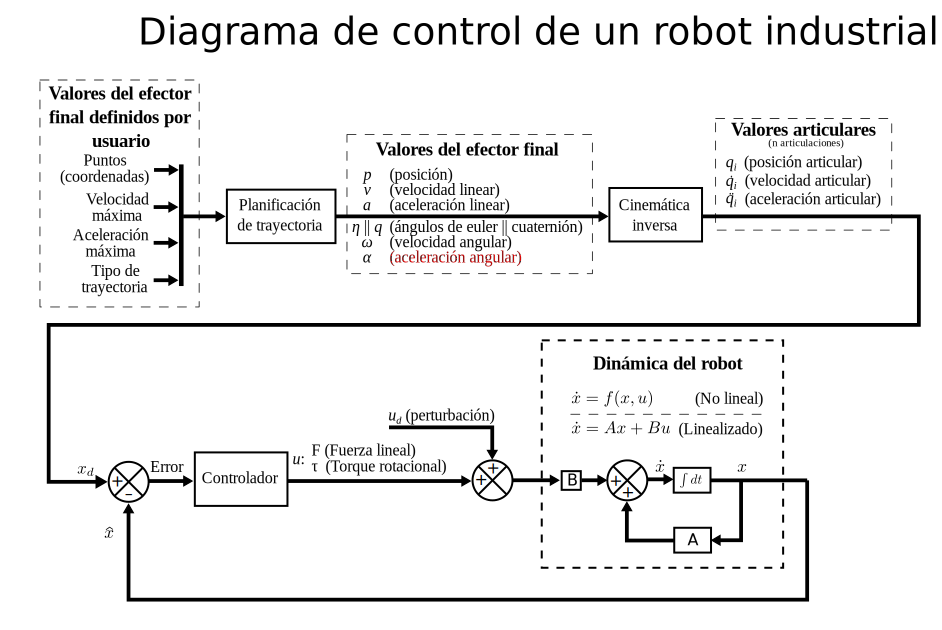
\includegraphics[width=\linewidth]{img/Diagrama_robot_industrial}
	\caption{Diagrama de bloques de un robot industrial}
	\label{fig:diagrama-de-robot-industrial}
\end{figure}

Después, se entra al bloque de dinámica del robot. Aquí se consideran los efectos físicos del movimiento, como la masa del robot, la inercia, las fuerzas y los torques necesarios para lograr el movimiento. También se toman en cuenta posibles perturbaciones externas que podrían afectar el comportamiento del robot, como fricción o impactos. El modelo dinámico puede analizarse en su forma más completa o como una versión simplificada y linealizada para facilitar el diseño del controlador.

El controlador compara el estado actual del robot con el estado que se desea alcanzar. Si hay diferencia, o error, el controlador genera una acción de control, que puede ser una fuerza o un torque, para corregir ese error. Todo este proceso ocurre de forma continua, actualizándose en tiempo real para asegurar que el robot siga la trayectoria correcta, incluso cuando existan perturbaciones o condiciones externas cambiantes.

En resumen, el diagrama muestra cómo se integra la información del usuario con las leyes del movimiento y el control automático para que el robot industrial pueda realizar tareas de manera precisa y eficiente.
\cite{fundamentosRobotica}
\cite{introduccionRobotica}




	
	% Capítulo 3: Desarrollo
	\chapter{Marco Teórico} 
\label{chap:marco_teorico}

La robótica es una rama de la ingeniería que estudia el diseño, construcción, operación y aplicación de robots, así como los sistemas computacionales que los controlan. Un robot es una máquina reprogramable capaz de realizar una serie de acciones automáticamente o por control externo, con cierto grado de autonomía. El estudio de los robots implica diversas áreas del conocimiento, entre ellas la mecánica, la electrónica, la programación y la teoría del control.

La cinemática se encarga del estudio del movimiento de los cuerpos sin considerar las fuerzas que los causan. En robótica, se distingue entre:

\textbf{Cinemática directa:} determina la posición y orientación del efector final en función de los valores articulares.

\textbf{Cinemática inversa:} calcula los valores articulares necesarios para alcanzar una posición deseada del efector.


El análisis cinemático es esencial para programar tareas de posicionamiento precisas en robots manipuladores.

La dinámica estudia el comportamiento del robot considerando las fuerzas involucradas en su movimiento. Permite calcular los torques o fuerzas necesarias para lograr un cierto movimiento bajo condiciones dinámicas. Este análisis es fundamental para el diseño del sistema de control y para garantizar que el robot pueda ejecutar tareas de manera estable y segura.
Las propiedades dinámicas de un robot incluyen:

\textbf{Inercia:} resistencia de las masas del robot al cambio de movimiento.

\textbf{Centrífugas y coriolis:} fuerzas que aparecen en sistemas en movimiento.

\textbf{Par gravitacional:} el efecto del peso del robot sobre sus articulaciones.

\cite{fundamentosRobotica}
\cite{introduccionRobotica}





	
		\section{Características del Robot} \label{sec:caracteristicas_del_robot}

En esta parte deben de explicar en una tabla la información principal del robot. Para ello, pueden cambiar el archivo de excel \ffile{Robot\_Resumen.xlsx} que está en \ffolder{tablas} y pedirle a ChatGPT que lo convierta a \LaTeX o simplemente pasarlo a un convertidor en línea.

\begin{table}[ht]
	\centering
	\caption{Parámetros de Denavit Hartenberg y límites del robot}
	\label{tab:parametros_robot}
	\begin{tabular}{ l|cccccccccccc
		}
		\toprule
		N & {$\theta$} & {$d$} & {$a$} & {$\alpha$} & {tipo} 
		& {$q_{\min}$} & {$q_{\max}$} 
		& {$\dot q_{\max}$} & {$\ddot q_{\max}$} 
		& {$\tau$} & {$\mu_s$} & {$\mu_k$} \\
		\midrule
		1 & 0 & 7 & 3  & 0   & r & -90 & 90 & 180 & 360 &  8  & 0.1 & 0.2 \\
		2 & 0 & 0 & 3  & -90 & r & -90 & 90 & 180 & 360 & 50  & 0.1 & 0.2 \\
		3 & 0 & 2 & 0  & -90 & r & -90 & 90 & 180 & 360 & 30  & 0.1 & 0.2 \\
		4 & 0 & 5 & 0  & 0   & p &   3 &  7 &   1 &   2 & 2  & 0.1 & 0.2 \\
		\bottomrule
	\end{tabular}
\end{table}
\bigskip
\noindent
\textbf{Donde (cambien las unidades):}
\begin{description}
	\item[N] Número de la articulación.
	\item[\(\theta\)] Ángulo articular (grados).
	\item[\(d\)] Desplazamiento articular (unidades de longitud).
	\item[\(a\)] Longitud del eslabón (unidades de longitud).
	\item[\(\alpha\)] Ángulo de torsión DH (grados).
	\item[tipo] ‘r’ para articulación rotacional, ‘p’ para prismática.
	\item[\(q_{\min}\), \(q_{\max}\)] Límites de posición (grados o unidades de desplazamiento).
	\item[\(\dot q_{\max}\)] Límite de velocidad (grados/s o unidades/s).
	\item[\(\ddot q_{\max}\)] Límite de aceleración (grados/s² o unidades/s²).
	\item[\(\tau\)] Torque o fuerza máxima permitido (\(N \cdot m\) o \(N\)).
	\item[\(\mu_s\)] Fricción estática (\(N\) o \(N \cdot m\)).
	\item[\(\mu_k\)] Fricción cinética (\(N \cdot m \cdot s\) o \(\frac{N \cdot m \cdot s}{rad}\)).
\end{description}


		
			\subsection{Partes} \label{subsec:partes}
Aquí pondrán la información de las piezas del robot. Pueden eliminar las siguientes subsecciones y simplemente explicar los motores usados y el material de los eslabones porque ya no hay tiempo.
\subsubsection{Motores} \label{subsubsec:motores}
Explicarán cuál es el motor que usaron, harán referencia a la hoja de datos, así como las transmisiones (por ejemplo, las de las pinzas) o reductores de velocidad a los que están acoplados. Deben de poner también información como: masa, fuerza o torque máximo, razón de reducción (por ejemplo, 10/1) y la velocidad máxima.
\subsubsection{Eslabones} \label{subsubsec:eslabones}
Pondrán la masa, inercia, longitud y material de cada eslabón.
			
			\subsection{Límites y propiedades dinámicas de las articulaciones} \label{subsec:limites_propiedades}


En la \autoref{tab:parametros_robot}: Parámetros de Denavit Hartenberg y límites del robot, se presentan los parámetros Denavit-Hartenberg (DH) y los límites de movimiento de cada articulación del robot. Los parámetros DH permiten describir matemáticamente la geometría del robot manipulador, utilizando una serie de transformaciones homogéneas que definen la relación entre cada eslabón.

La columna tipo especifica el tipo de articulación, donde “r” indica que es rotacional (revoluta). Además, se incluyen los límites de movimiento: qmin y qmax representan el rango angular permitido para cada articulación, q'max indica la velocidad angular máxima, y q''max señala la aceleración angular máxima permitida. Estos valores son fundamentales para garantizar que el robot opere dentro de márgenes seguros, evitando sobrecargas o colisiones durante su funcionamiento.

		
		Aquí explicarán su código
Si quieren mostrar un código, pueden hacerlo de la siguiente forma

\begin{minted}{matlab}
	function [q_sol, p_sol] = cinematica_inv(r, p_des, tol, max_iter, alpha, numMuestras)
\end{minted}

Si les sale el error \texttt{latexminted no se reconoce como un comando interno o externo, programa o archivo por lotes ejecutable}, pueden usar 
\begin{terminal}{Instalar minted en python con pip}
	pip install latexminted==0.5.1
\end{terminal}

		
		\section{Control}
El diagrama de control de un robot industrial representa cómo se procesa la información desde que el usuario define lo que quiere que haga el robot, hasta que este ejecuta el movimiento real. Se puede dividir en tres bloques principales: la planificación de trayectoria, la cinemática inversa y la dinámica del robot.

Primero, el usuario define los valores que quiere que alcance el efector final del robot. Estos valores pueden ser las coordenadas de los puntos que debe seguir, la velocidad máxima, la aceleración máxima y el tipo de trayectoria. Esta información entra al bloque de planificación de trayectoria, donde se generan los valores que describen cómo debe moverse el efector final, como su posición, velocidad y aceleración, tanto lineal como angular.

Luego, esta información pasa a la parte de la cinemática inversa. Ahí se transforma en variables articulares, es decir, se calculan las posiciones, velocidades y aceleraciones que deben tener las articulaciones del robot para que el efector final logre seguir correctamente la trayectoria deseada.



\begin{figure}[h]
	\centering
	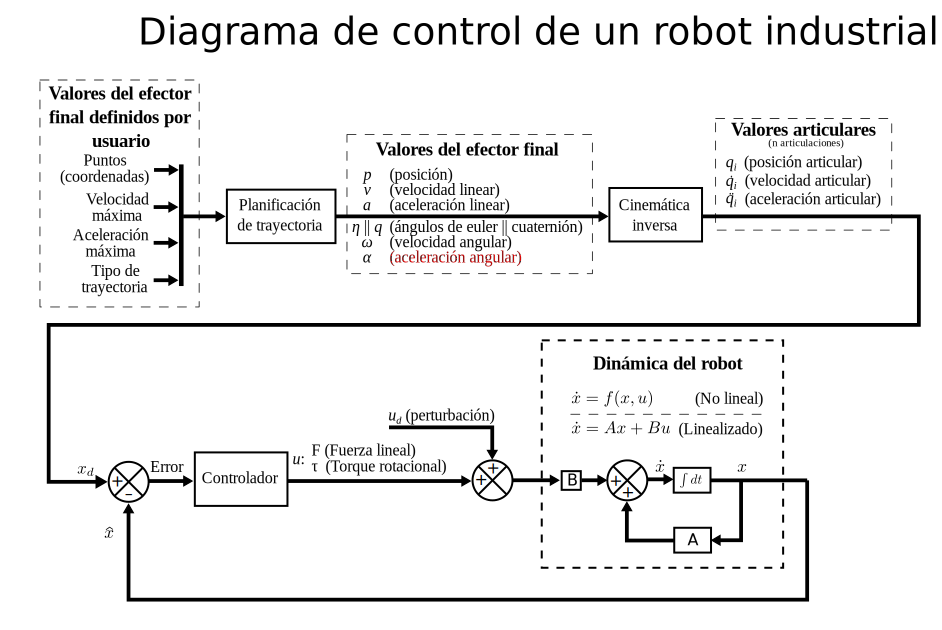
\includegraphics[width=\linewidth]{img/Diagrama_robot_industrial}
	\caption{Diagrama de bloques de un robot industrial}
	\label{fig:diagrama-de-robot-industrial}
\end{figure}

Después, se entra al bloque de dinámica del robot. Aquí se consideran los efectos físicos del movimiento, como la masa del robot, la inercia, las fuerzas y los torques necesarios para lograr el movimiento. También se toman en cuenta posibles perturbaciones externas que podrían afectar el comportamiento del robot, como fricción o impactos. El modelo dinámico puede analizarse en su forma más completa o como una versión simplificada y linealizada para facilitar el diseño del controlador.

El controlador compara el estado actual del robot con el estado que se desea alcanzar. Si hay diferencia, o error, el controlador genera una acción de control, que puede ser una fuerza o un torque, para corregir ese error. Todo este proceso ocurre de forma continua, actualizándose en tiempo real para asegurar que el robot siga la trayectoria correcta, incluso cuando existan perturbaciones o condiciones externas cambiantes.

En resumen, el diagrama muestra cómo se integra la información del usuario con las leyes del movimiento y el control automático para que el robot industrial pueda realizar tareas de manera precisa y eficiente.
\cite{fundamentosRobotica}
\cite{introduccionRobotica}




		
		\input{capitulos/Desarrollo/Simulación}
	
	% Capítulo 4: Resultados
	\chapter{Resultados} \label{chap:resultados}
Aquí pondrán las gráficas que obtuvieron en la simulación de matlab para el robot (si las tienen), y las explicarán.

También mostrarán capturas de pantalla de cómo se ve en Gazebo el robot y en RViz, ya sea que funcione o no, para el cambio de trayectoria. Describirán lo que ocurre y por qué (si es que saben).

	
	% Capítulo 5: Conclusiones
	\chapter{Conclusiones} \label{sec:conclusiones}
	\section{Ceballos Portillo, Patsy}
El desarrollo y análisis de la cinemática diferencial del robot manipulador permitieron comprender de manera profunda el comportamiento dinámico del sistema en función del tiempo y las variables articulares. A través del cálculo preciso del Jacobiano geométrico y su derivada temporal, se logró establecer una relación directa entre las velocidades articulares y las velocidades lineales y angulares del efector final. Este proceso es fundamental no solo para simular correctamente el movimiento del robot, sino también para diseñar estrategias de control más avanzadas, como el control de trayectoria o el seguimiento en tiempo real. La obtención y representación gráfica de la velocidad y aceleración del efector en los tres ejes cartesianos permitieron validar el correcto funcionamiento del algoritmo, identificar posibles inconsistencias y evaluar el comportamiento esperado de la trayectoria. Estas gráficas no solo son una herramienta de validación técnica, sino también un recurso visual que facilita la interpretación de los resultados por parte de estudiantes, docentes e ingenieros, fortaleciendo así el puente entre la teoría matemática de la robótica y su aplicación práctica en simulaciones computacionales.
	\section{Panchito}
Conclusiones y comentarios de Panchito, explicando los problemas que tuvo y lo que aprendió.
	\section{Lupita}
Conclusiones y comentarios de Lupita, explicando los problemas que tuvo y lo que aprendió.
	\section{Peña Encinas, Ana Lourdes}
Durante el proceso de implementación del código, se evidenció la importancia de estructurar correctamente cada bloque funcional, desde la definición de la cinemática hasta la generación de la animación. Especialmente, se identificó el papel central que desempeñan el Jacobiano y su derivada en la interpretación del comportamiento cinemático del robot en el espacio operacional. Estas matrices no solo permiten traducir los movimientos articulares a movimientos del efector, sino que también sirven como base para entender cómo pequeñas variaciones en las articulaciones impactan en la trayectoria del extremo del robot. El hecho de que este análisis se haya complementado con gráficas detalladas de posición, velocidad, aceleración y orientación permitió una evaluación mucho más completa del sistema. Además, se hizo evidente la utilidad de contar con una estructura modular en el código, en donde cada función realiza una tarea específica y puede reutilizarse o modificarse de forma sencilla. Este enfoque de programación no solo facilita la comprensión del algoritmo, sino que también permite su extensión hacia sistemas más complejos o con mayores grados de libertad.
		
	\titleformat{\chapter}
	{\bfseries\huge}
	{}
	{0pt}
	{~\raisebox{-1.5pt}{}
		\\\vspace{.05cm}\titlerule\\\filcenter #1 \\\vspace{.25cm}\titlerule}
	%{\titlerule\\\vspace{.25cm}\filcenter #1 \\\vspace{.25cm}\titlerule}
	\bibliographystyle{IEEEtranN}
	\newpage\label{bibliografia}
	\addcontentsline{toc}{chapter}{Bibliografía}
	
	% Pulsa Ctrl + Clic Izquierdo en bibliografia para entrar.
	\bibliography{bibliografia}
\end{document}


